%!TEX root = root.tex
The generation of whole-body motions using multiple contacts between the robot and its environment extends the form of bipedal locomotion with a potential high impact on humanoid robot functionalities.
It enables a robot to climb ladders, crawl, evolve in cluttered environment and less impressively, but yet very useful, climb stairs \cite{Tedrake:ichr:2014, Keddar:iros:2014}.
Staircase climbing is an important basic behavior for humanoid robots aiming at evolving in an industrial environment (see Fig.~\ref{fig:covermultimanuel}).
The DARPA Robotics challenge has illustrated the difficulty of this realization.
%Among several problems, a crucial one for DC-motor-based humanoid robot is the power consumption.
%
\begin{figure}[t]
  \centering
  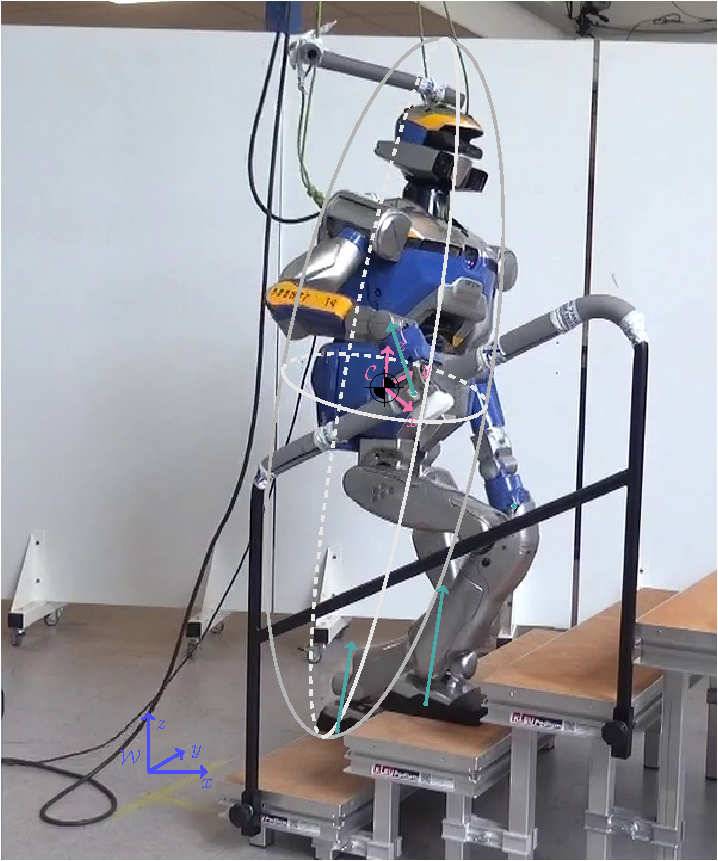
\includegraphics[width=0.35\linewidth, keepaspectratio,trim=50pt 20pt 10pt 10pt,clip=true]{./figures/cover.pdf}%
  \caption{HRP-2 climbing stairs with the support of the handrail.
The overlay shows the reduced model (center of mass (CoM, black) at waist, CoM frame (magenta), gray inertia ellipsoid, contacts (teal dots) and contact forces (teal arrows) as well as world coordinate system $\mathcal W$ (blue).}
  \label{fig:covermultimanuel}
\end{figure}
%
% \begin{figure}[t]
%   \centering
%   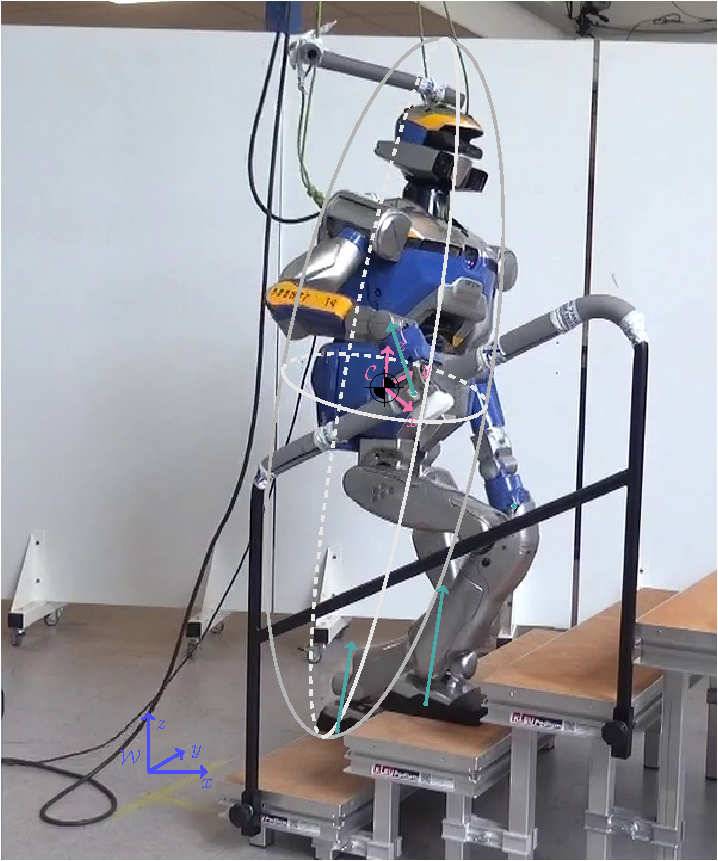
\includegraphics[width=1.0\linewidth, keepaspectratio]{%
%       ./figures/tikz/reduced_model_setup_with_hrp2.pdf%
%   }
%   \caption{%
%   Simulation of HRP-2 climbing stairs with support of a handrail using Pinnochio~\cite{pinocchio:laas}.
%   The overlay shows the used reduced model (center of mass (CoM, black) at waist, CoM frame (magenta), gray inertia ellipsoid, contacts (teal dots) and contact contact forces (teal arrows) as well as world coordinate system $\mathcal W$ (blue).}
%   \label{fig:openhrp_setup}
% \end{figure}
Two main classes of approaches can be distinguished in the resolution of the multi-contact locomotion problem.
On the one hand, the problem is approached all at once, by trying to find a complete trajectory of the system typically using a numerical resolution scheme.
On the other hand, the problem is decomposed into several sub problems, typically by following the seminal approach used in ground-level bipedal locomotion.

Ideally, multi-contact motion generation includes a dynamic model of the humanoid, a model of its actuators and takes into account all its constraints over a finite preview-window.
The number of degrees of freedom~(DoFs) and the size of the needed preview-window make this approach useful for motions \cite{Koch2012a} exploiting the whole robot, but its computational complexity prevents an execution in real-time.

The first class of approaches mostly tries to make the problem tractable by proposing various ways of approximating the complete problem or improving the mathematical properties arising from a specific formulation.
\cite{Tedrake:ichr:2014} proposed to work on the under-actuated dynamics and consider only the constraints related to inverse kinematics.
\cite{Todorov:ICRA:2014} proposed to reformulate the contact model, and use differential dynamic programming to solve the related optimization problem efficiently.
In practice, the contact model is sufficient for transition with the robot hands for object reaching for example.
But for walking, the contact model gives inconsistent data which results in unwanted or unbalanced behavior, like walking on the feet edges.

The authors of \cite{herzog2015trajectory} implemented a planner for the linear and angular momentum taking into account multiple contacts.
They used friction cones and solved the problem using SQP methods linearizing the dynamics.
The tracking of the spatial momentum is done via an LQR providing the ankle wrench to a low level torque controller.
This planner computes dynamically consistent multicontact trajectories but in around $5\,min$.
Hence it is not suitable for real time motion generation.

Another approach is presented in \cite{Hirukawa:icra:2007}, where the authors consider a set of contact points for which a dynamically consistent CoM trajectory is found.
The forces are subject to the linearized friction cone constraints.
This iterative algorithm assumes a predefined partitioning of the external forces applied to the system.
In \cite{Ott:Humanoids:2011} a stabilization process based upon the work of Cheng~\cite{DBLP:journals/trob/HyonHC07} is proposed.
They propose to handle contact forces via the Coulomb friction cone typically used in grasping.
They design a force based stabilizer that take into account the CoM dynamics and the joint position.
It assumes a quasi-static joint motion, i.e. joint accelerations and velocity are assumed to be zero to map the external wrench to the joint torques.
This condition imposes restrictions on the possible motions.
%
%
%Requirement for a successful achievement of these tasks in reality are methods that can solve these problems efficiently and fast. This is still the scope of current research.
%

3D walking, i.e. stair walking or stepping stone, has already been investigated by the community.
\cite{Kajita:icra:2003} shown that simple CoP control can be used in simulation to climb stairs.
\cite{naveau:ichr:2014} shown that the dynamic filter, i.e. the second stage of Kajita, allows to take into account the whole body dynamics while climbing the stairs.
In \cite{englsberger:iros:2015} the author proposed a 3D extension of the capture point.
They formalized the non stable part of the linear inverted pendulum dynamics as a 3D point.
They show uneven ground walking and stair climbing motion controlling this point dynamics.
All these algorithms plan the CoM trajectories for either predefined or online computed foot contacts.
Extensive simplifications of the humanoid dynamic model result in a linear inverted pendulum model, which allows the fast generation of walking motions.
The extensions proposed in \cite{Nishiwaki:IJRR:2012} can handle steep slopes of $10^\circ$ and show the humanoid robot platform HRP-2~\cite{Kaneko2004} hitting obstacles and appropriately adapting its feet trajectory.

While these simplified models have a small computational footprint and show consistency with the elementary parts of the human gait, they all assume zero variation of the angular momentum about the CoM, which is once more a strong limitation for achieving complex dynamic movements.
In practice having zero variation of the angular momentum about the CoM means that a parallel controller use the free DoFs to cancel this variation of the angular momentum impose by the controlled DoFs.
Typically while walking the legs impose a momentum on the CoM and a swing motion of the robot arms can be used to cancel this momentum.
These angular effects can be integrated directly inside the dynamic model based on the centroidal momentum described in~\cite{Orin:autorob:2013}.
It consist in modeling the robot as rigid body with a constant inertia.
Hence, the variation of angular momentum created by contacts between the robot and its environment on the CoM can be approximated.
Thereby, the robot is model using the centroidal momentum.
%
%
%
%The previously cited approaches project the dynamics of the humanoid on its CoM.
%Other approaches to walking motion generation try to take a model of the full dynamics of the kinematic chain.
%In \cite{tassa_control-limited_2013},\cite{tassa:icra:14} methods of differential dynamic programming are used to generate different whole body motions using full dynamic models of humanoids.
%By considering the full dynamic model of the humanoid the applied methods have a high computational cost and have not yet been used as controllers on real humanoid robots.

\subsection*{Contribution of the chapter}

\begin{itemize}
\item It proposes a mathematical formulation of the reduced multi-contact CoM dynamics of a humanoid as an optimal control problem~(OCP).
\item It experimentally shows that the humanoid robot platform \mbox{HRP-2} is able to climb stairs with a handrail support using this approach.
\item It demonstrates from experimental study on the robot that handrail support reduces the motor power consumption by $25\%$.
\end{itemize}

The OCP is able to find feasible CoM trajectories and contact forces for predefined contact sets.
The constraints are the contact model and the kinematic limits of the whole-body system.
The template model includes the major effects on the under-actuated part and is applicable for any combination of contact (ground level, biped walk on non-flat floor, multi-contact like using the handrail during stair climbing, etc).
In collaboration with Steve Tonneau, we computed the contact sequences using his multicontact planner presented in \cite{tonneau_isrr15}.
The following scheme Fig.~\ref{fig:overview_joint_trajectories} present the architecture of the controller.

\begin{figure}[ht]
\vspace*{0.3cm}
\begin{center}
\tikzstyle{MGstyle} =[text centered,draw=blue!50,fill=blue!20,thick,]
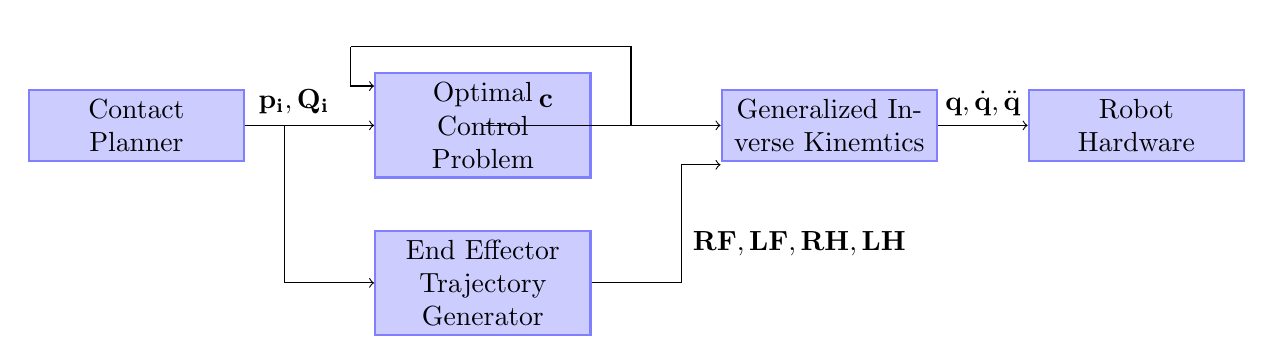
\begin{tikzpicture}[font=\normalsize, node distance=1cm]
% The boxes
  \node (cp)   at (0,0) [shape=rectangle,MGstyle,text width=2.5cm]
  {Contact Planner};
  
  \node (eetg)   at (4.4,-2.0) [shape=rectangle,MGstyle,text width=2.5cm]
  {End Effector Trajectory Generator};

  \node (ocp)  at (4.4,0) [MGstyle,text width=2.5cm]
  {Optimal Control Problem};

  \node (gik) at (8.8,0) [MGstyle,text width=2.5cm]
  {Generalized Inverse Kinemtics};
  
  \node (robot)  at (12.7,0) [MGstyle,text width=2.5cm]
  {Robot Hardware};
% The arrows
  % forward
  \draw [->] (cp) -- node [xshift=-0.2cm,yshift=0.3cm] {${\bf p_i},{\bf Q_i}$} (ocp);
  \draw [->] ([xshift=0.5cm]cp.east) |- node {}([xshift=-0.2cm]eetg); 
  \draw [->] (ocp) |- node [xshift=0.8cm,yshift=0.3cm] {${\bf c}$}(gik);
  \draw [- ] (eetg) -| node [xshift=1.5cm,yshift=0.5cm]{${\bf RF},{\bf LF},{\bf RH},{\bf LH}$}([xshift=-0.5cm,yshift=-0.5cm]gik.west);
  \draw [->] ([xshift=-0.5cm,yshift=-0.5cm]gik.west) -- node {}([yshift=-0.5cm]gik.west);
  \draw [->] (gik) -- node [above] {${\bf q}, \dot{\bf q}, \ddot{\bf q}$} (robot);  

  % feedback
  \draw [- ] ([xshift=0.5cm]ocp.east) |- node [above] {} ([xshift=-0.3cm,yshift=1cm]ocp.west);  
  \draw [->] ([xshift=-0.3cm,yshift=1cm]ocp.west) |- node {} ([yshift=0.5cm]ocp.west);
  
\end{tikzpicture}
\end{center}
\caption{Overview of the joint trajectories (${\bf q}$) generation process, with 
${\bf p_i},{\bf Q_i}$ the contact positions and orientations,
${\bf c}$ the CoM trajectory,
and ${\bf RF},{\bf LF},{\bf RH},{\bf LH}$ the end-effector trajectories.}
\label{fig:overview_joint_trajectories}
\end{figure}